%!TeX program=pdflatex
%!TeX encoding=utf8
%!TeX spellcheck = en_US
%!TeX root = ../../messageVortex.tex


% ********************************************************************************************************
% *** Intro
% ********************************************************************************************************


\chapter{Our Contribution}
This thesis contributes to anonymization with an asynchronous messaging protocol called MessageVortex.

The protocol employs a new type of programmable forwarders called ``routing nodes'' (nodes) with a novel way of message mixing, moving away from a strictly chunked and onionized system, to a system where routing operations allow to increase or decrease in size without differentiating between decoy traffic and message routing. We refer to the instructions required to process a node as ``routing blocks''. These routing blocks have an onionized structure, only exposing the required information for the current node. Routing blocks may travel with a message or join at any common routing node with the message.

To non-traceable routing this, we introduce a novel type of routing operation called ``addRedundancy''. This operation is a Reed-Solomon-calculation with encryption and a new type of padding. This operation transposes the received information in a form bigger or smaller than the original message by adding or removing redundancy operations. The applied padding structures the message in such a way that any possible result of a decryption operation results in a plausible padding structure. With standard paddings, decoy operations on traffic would possibly be identifiable as the resulting padding structure may be invalid leaking information. After applying these operations, the routing node then sends this transposed information to subsequent peers without any knowledge of what parts of the sent messages are relevant for the successful message delivery. Therefore, applying such operations makes it impossible for any node to differentiate between decoy traffic and real message traffic. Furthermore, tagging beyond peering nodes is not possible, as building relations between messages of non-neighboring nodes is not possible.

An outside observer is unable to identify messages, as they do not use proprietary communication protocol but hide within other standard internet protocols. We blend these transport protocols without modifying the servers used for message transport. This property makes the protocol very robust as the prosecution of server administrators is not sensible if traffic is running over their infrastructures. 

As the structure of routing blocks does not expose the encryption keys required to build routing blocks for a peering node, a malicious node may only discover other possible peer partners when routing traffic without gaining the capability of talking to them. Other properties, such as type of routed traffic, message size, message content, communication partners, or intensity of communication, remain hidden. External global observers are unable to differentiate between regular protocol traffic and Vortex traffic. Assuming an observer capable of identifying the steganographically hidden information, he may apply censorship but remains unable to trace messages according to externally attributes, even assuming that he has additional information from collaborating nodes within the message path.

Our protocol differentiates from other protocols by the fact that our way of mixing and routing messages does not rely on knowingly injected decoy traffic and that we are capable of piggybacking multiple other carrier protocols without modifying the required, already available infrastructure on the internet or requiring dedicated infrastructure. The carrier protocols may even be switched during routing, making it even harder to observe message traffic.


\chapter{Overview over Existing Implementations and Research on the Topic}
\fxwarning{Get summary from old document}

\chapter{Main Research Question}
The main topic of this thesis was defined as follows:
\begin{itemize}
	\item Is it possible to have a specialized messaging protocol used on the Internet-based on ``state of the science'' technologies offering a high level of unlikability (sender and receiver anonymity) towards an adversary with a high budget and privileged access to Internet infrastructure?
\end{itemize}

Based on this central question, there are several sub-questions grouped around various topics:

\begin{enumerate}
	\item What technologies and methods may be used to provide sender and receiver anonymity and unlinkability when sending messages against a potential adversary? (SQ1)
	\item How can entities utilizing \emph{MessageVortex} be attacked, and what measures are available to circumvent such attacks? (SQ2)
	\item How can design mitigate attacks target anonymity of a sending or receiving entity within \emph{MessageVortex}? (SQ3)
\end{enumerate}

\section{SQ1: Technologies for Sending Messages Maintaining Unlinkability}
This question covers the principal part of the work. We first elaborate on a list of criteria for the \emph{MessageVortex} protocol. We then create a list of suitable technologies and methods. Based on these findings, we define a protocol combining these technologies and researches into a solution. This solution is implemented and analyzed for suitability based on the criteria specified previously.

Main results of this question are found in part~\ref{sec:methodes} and part~\ref{sec:results}.

\section{SQ2: Attacking unlinkability and circumvention}
Within this question, we look at various attacks and test resistance of the protocol based on the definition of the protocol. We do this by first collecting well-known attacks (either generic or specific to a technology used in the protocol). We then elaborate if those attacks might be successful (and if so under what circumstances).

We discuss this question in part~\ref{sec:discussion}.

\section{SQ3: Attack Mitigation by design}
Within this question, we define baselines to mitigate attacks by identifying guidelines for using the protocol. We analyze the effectiveness of the guidelines and elaborate on the general achievement level of the protocol by looking again at the criteria defined in SQ1. 

This question is answered in part \ref{sec:discussion}.

% ********************************************************************************************************
% *** Intro to MessageVortex
% ********************************************************************************************************
% ********************************************************************************************************
% *** Research Preexisting work
% ********************************************************************************************************
\part{Related Work}
\fxwarning{complete section}
\chapter{Anonymity Research}
In this section, we collect protocols research related to anonymity. We did not stick to anonymous message transfer. Instead, we took a broad focus in terms of technology and outlined in each protocol strengths and weaknesses identified, which may be relevant to this research.

\section{Definition of Anonymity}
As the definition for Anonymity we take the definition as specified in \cite{anonTerminology}.\DeclareFixedFootnote{\omitted}{footnotes omitted in quote}
\begin{quote}
	Anonymity of a subject means that the subject is not identifiable within a set of subjects, the anonymity set.\omitted
\end{quote}
and
\begin{quote}
	Anonymity of a subject from an attacker's perspective means that the attacker cannot sufficiently identify the subject within a set of subjects, the anonymity set.\omitted
\end{quote}

We define the anonymity set as the set of all possible subjects within a supposed message. The anonymity of a subject towards an observing third party is a crucial factor as it relates directly to our adversary model.

\section{$k$-Anonymity}
\fxwarning{complete section}
\section{$\ell$-Anonymity}
\fxwarning{complete section}
\section{$t$-closeness}
\fxwarning{complete section}
\section{Single and Multi Use Reply Blocks}
\fxwarning{complete section}
\chapter{Censorship}
\fxwarning{complete section}
\section{Censorship Resistance}
\fxwarning{complete section}
\section{Censorship Circumvention}
\fxwarning{complete section}
\section{Parrot Circumvention}
\fxwarning{complete section}

\chapter{Cryptography and Steganography}
\fxwarning{complete section}
\section{Homomorphic Encryption}
\fxwarning{complete section}
\section{Deniable Encryption}
\fxwarning{complete section}
\section{Deniable Steganography}
\fxwarning{complete section}
\section{Cryptographic modes for Block Cyphers}
\fxwarning{complete section}
\section{Padding for Block Cyphres}
\fxwarning{complete section}

\chapter{Information Routing and Distribution for Anonymizing Protocols}
\fxwarning{complete section}
\section{Mixing}
\fxwarning{complete section}
\section{Onionizing}
\fxwarning{complete section}
\section{Mimic Routes}
\fxwarning{complete section}
\section{Distributed Hash Tables}
\fxwarning{complete section}
\section{Dining Cryptographer Networks}
\fxwarning{complete section}

\chapter{Proposed Academic Protocols and System Implementations}
\fxwarning{complete section}
\section{Characteristics of Known Anonymity Implementations}
Table \ref{tab:anonClass} shows the previously analyzed protocols.

\begin{table*}[t]\centering\tiny
	\label{tab:anonClass}
	\setlength{\aboverulesep}{0pt}
	\setlength{\belowrulesep}{0pt}
	\newcolumntype{x}[1]{!{\centering\arraybackslash\vrule width #1}}
	% network
	%\usepackage{ amssymb }
	\newcommand\fullyn{$\boxtimes$}
	\newcommand\mostlyn{$\square$}
	\newcommand\partlyn{$\sqsubset$}
	%direction
	\newcommand\bidi{$\longleftrightarrow$}
	\newcommand\unidi{$\longrightarrow$}
	% synchronization
	\newcommand\async{$\neq$}
	\newcommand\sync{$\cong$}
	% symmetry
	\newcommand\ptp{\scalebox{0.4}{$\bullet\cdots\bullet\cdots\bullet$}}
	\newcommand\cs{\scalebox{0.4}{$\bullet\cdots\bullet$}}
	\newcommand\hybrid{\scalebox{0.4}{$\bullet\cdots\circ\cdots\bullet$}}
	% Hierarchy
	\newcommand\flath{$\cdots$}
	\newcommand\hierarch{\ding{68}}
	% centralization
	\newcommand\partcentr{\astrosun}
	\newcommand\decentr{$\circ$}
	% Network view
	\newcommand\fullynv{$\CIRCLE$}
	\newcommand\partlynv{$\LEFTcircle$}
	% NW updating
	\newcommand\timed{\clock}
	\newcommand\event{\lightning}
	\newcommand\noupd{\ding{56}}
	% Routing
	\newcommand\routesrc{\scalebox{0.4}{$\bullet\cdots$}}
	\newcommand\routehop{\scalebox{0.4}{$\cdots\bullet\cdots$}}
	\newcommand\routebc{\faBullhorn}
	% Routing
	\newcommand\shedfair{$\equiv$}
	\newcommand\shedprio{$\Diamonddot$}
	%determinism
	\newcommand\nsdetdet{\checkmark}
	\newcommand\nsdetprob{$\ding{56}$}
	%determinism
	\newcommand\nsnodesall{\CircledA}
	\newcommand\nsnodessec{\Stopsign}
	\newcommand\nsnodesnet{\Mundus}
	\newcommand\nsnodesusr{\smiley}
	% probability
	\newcommand\nsprobuni{$\circledast$}
	\newcommand\nsprobstat{$\circledcirc$}
	\newcommand\nsprobdyn{$\ast$}
	% latency
	\newcommand\perflatl{L}
	\newcommand\perflath{H}
	\newcommand\perflatm{M}
	% mode 
	\newcommand\perfmodecon{$\multimapdotboth$}
	\newcommand\perfmodemsg{$\Letter$}
	% implementation
	\newcommand\nsimplyes{\checkmark}
	\newcommand\nsimplno{$\ding{56}$}
	% code available
	\newcommand\nscodeyes{\checkmark}
	\newcommand\nscodeno{$\ding{56}$}
	% context
	\newcommand\nscontmsg{\faEnvelope}
	\newcommand\nscontmail{@}
	\newcommand\nscontbulletin{\faUsers}
	\newcommand\nscontphone{\Telefon}
	\newcommand\nscontwww{\faInternetExplorer}
	\newcommand\nscontmicroblog\faPencil
	\newcommand\nscontfiles\faStickyNote
	\newcommand\nscontwifi\faWifi
	\gdef\cwidth{0.37cm}
	\rowcolors{8}{black!30}{black!10}
	\begin{tabular}{x{2pt}lx{2pt}*{5}{p{\cwidth}|}p{\cwidth}x{2pt}p{\cwidth}|p{\cwidth}x{2pt}*{4}{p{\cwidth}|}p{\cwidth}x{2pt}*{4}{p{\cwidth}|}p{\cwidth}x{2pt}}
		\toprule
		
		& \multicolumn{6}{cx{2pt}}{Network Structure} & \multicolumn{2}{p{1.2cm}x{2pt}}{\centering Routing Information} & \multicolumn{5}{cx{2pt}}{Communication Model} & \multicolumn{5}{cx{2pt}}{Performance and Deployability}\\\cmidrule{2-19}
		
		& & \multicolumn{2}{c|}{Connection} & \multicolumn{3}{cx{2pt}}{Symmetry} & & & & & \multicolumn{3}{cx{2pt}}{Node Selection} & & & & & \\\cmidrule{3-4}\cmidrule{5-7}\cmidrule{12-14}
		
		& \rot{Topology} & \rot{Direction} & \rot{Synchronization} & \rot{Roles} & \rot{Hierarchy} & \rot{Decentralization} & \rot{Network view} & \rot{Updating} & \rot{Routing Type} & \rot{Scheduling} & \rot{Determinism} & \rot{Selection set} & \rot{selection probability} & \rot{Latency} & \rot{Communication mode} & \rot{Implementation} & \rot{Code availability} & \rot{Context/application} \\
		\midrule
		MessageVortex & \fullyn & \bidi & \async & \ptp & \flath & \decentr & \partlynv &  \event &  \routesrc & \shedfair & \nsdetprob & \nsnodesusr & \nsprobuni & \perflath & \perfmodemsg & \nsimplyes & \nscodeyes & \nscontmail \\
		Riffle & & & & & & & & & & & & & & & & & & \\
		Atom & & & & & & & & & & & & & & & & & & \\
		Riposte & & & & & & & & & & & & & & & & & & \\
		Pung & & & & & & & & & & & & & & & & & & \\
		PIR & & & & & & & & & & & & & & & & & & \\
		Karaoke & & & & & & & & & & & & & & & & & & \\
		Loopix & & & & & & & & & & & & & & & & & & \\
		Stadium & & & & & & & & & & & & & & & & & & \\
		Vuvuzela & & & & & & & & & & & & & & & & & & \\
		\bottomrule
	\end{tabular}
	\caption{Classification table for anonymization protocols according to \cite{Shirazi2018}}
\end{table*}

\section{Remailers, Resenders, Onion Routers, and Mixnets}
\subsection{Pseudonymous Remailers (1981)\label{sec:remPseudo}}
The basic idea of remailers was discussed in \cite{CHAUM1}. The most well-known remailer was probably anon.penet.fi, which operated from 1993 to 1996. This type of remailer is often referred to as type-0-remailer.

In principle, an anonymous remailer works as an ordinary forwarding service for messages (e.g., \defref{SMTP}). The only difference is that it strips off all meta information and then replaces the sender and recipient address with pseudonyms respectively with the real address. 

This kind of remailer is easily attackable by an authority. The remailer has a directory containing the tuples of pseudonyms and their respective real identities. Such a list breakes effectively anonymity or pseudonymity even retrospectively if obtained by an adversary. To giv an example, this was the case in the closure of penet remailer\cite{penetClosure}. Furthermore, the message may be monitored at the server or on its way, and then due to the unmodified content matching is easy.

This remailer offers, therefore, no protection against an adversary defined in our problem.

\subsection{Cypherpunk Remailers (approx. 1993)\label{sec:remCypherpunk}}
With the failing of anon.penet.fi, it became clear that the weakest spot of a single server infrastructure the information stored on the server and the vulnerability of their owner. The new type-1-remailers score over the existing type-0-remailers by using encryption for the message. Most of the time PGP was used and custom programmed mail processors on systems to achieve the functionallity. It is unclear when first type-1-remailers were invented. Setting up a type-1-remailer was typically achieved by using procmail together with a small script calling PGP binaries and then sending the resulting message to the next recipient. By combining multiple type-1-remailers, an onion-like structure of the message was achievable. 

This approach was promising, but it was still observable. An observation was possible by correlating the message sizes (e.g., strictly decreasing) and timing information. Furthermore, remailers were however still known and authorities were able to ban infrastructure and capable of monitoring their routing activities. Additionally, those remailers allowed to prosecute administrators of such systems.

\subsection{Babel (1996)}
Babel was an academic system defined in a paper by \citeauthor{babel} in \citeyear{babel}\cite{babel}. It has been developed at IBM Zurich Research Laboratory. It was a mixing system using onionized addresses. The sender remains anonymous while he may provide a reply routing block called RPI. If both parties would like to remain anonymous, the RPI of the initiator is deployed in a forum thread. Anyone using this block adds an RPI for its address to the message.

This system has all the disadvantages of a system using MURBs. Traffic highlighting and similar attacks are possible.

\subsection{Mixmaster-Remailers (1996)\label{sec:remMixmaster}}
Like Cypherpunk remailers, the Mixmaster remailers were working with onion-like encrypted messages. The protocol was based on Mix-Nets described by Chaum in \cite{CHAUM1} and further developed by L. Cotrell in 1996. 

In contrast to type-1-remailers, the use of cascading systems to remail became systematic. The enduser used specialized software to build and send Mixmaster messages.

Mixmaster messages were still traceable by message size. Reply blocks were not supported by the system. A user had to know all Mixmaster nodes in order to use the system. The last node was typically an exit node sending the message in clear to the final recipient. This behavior still allowed the use of Usenet.

\subsection{Crowds (1997)}
\fxwarning{insert jondosystem}

\subsection{Tor (2000)\label{sec:tor}}
Tor is one of the most common onion router networks these days and onionizes generic TCP streams. It is specified in \cite{tor-spec}. It might be considered one of the most advanced networks since it has a considerable size, and much research has been done here.

According to \cite{onion-routing:pet2000} Tor is a network consisting of multiple onion routers. Each client first picks an entry node. Then it establishes an identity, gets a listing of relay servers, and chooses a path through multiple onion routers. The temporary identity links to such a path and should be changed on a regular base along with its identity. Transferring data works by splitting the data into equally sized cells of 512 bytes.

There is a centrally organized directory in the Tor network, knowing all tor relay servers. Any Tor relay server may be a directory server as well. 

Many attacks involving the Tor networks have been discussed in the academic world such as \cite{hs-attack06,esorics13-cellflood,bauer:wpes2007,esorics12-torscan,oakland2013-trawling,danner-et-al:tissec12,congestion-longpaths} and some have even been exploited actively. In the best case, the people discovering the attacks did propose mitigation to the attack. Some of these mitigations flowed back into the protocol. Some general thoughts of the attacks should be emphasized here for treatment in our protocol.

Being an exit node may be a problem in some jurisdictions. In general, it seems to be accepted that routing traffic with unknown content (to the routing node) is not regarded as illegal per se. So by being unable to tell malicious or illegal traffic apart from legitimate traffic, this is not a problem. However -- being an exit node can mean that unencrypted and illegal traffic is leaving the routing traffic. In this specific case, operators of a relay node might fear legal prosecution. Tor nodes may proclaim themselves as  `` non-exit nodes''  to avoid the possibility of legal prosecution.

Furthermore, several DoS-Attacks have been carried out to overload parts of the Tor network. Most of them do a bandwidth drain on the network layer.

Attacking anonymization has been done in several ways. First of all, the most common attack is a time-wise correlation of packets if in control of an entry and an exit node. A massive attack of this kind was published in 2014 and has been published on the tor website (\href{https://blog.torproject.org/blog/tor-security-advisory-relay-early-traffic-confirmation-attack}{relay early traffic confirmation attack}). This attack was possible because tor is a low latency network. Another attack is to identify routes through tor by statistically analyze the traffic density in the network between nodes. More theoretical attacks focus on the possibility of controlling the directory servers to guarantee that an entity may be deanonymized because it is using compromised routers.

Generally, the effectiveness of the monitoring of single nodes or whole networks is disputed. According to a study by \citeauthor{ccs2013-usersrouted} in \citeyear{ccs2013-usersrouted}\cite{ccs2013-usersrouted}, a system in the scale of PRISM should be able to correlate traffic of 95\% of the users within a ``few days''. Other sources based on the Snowden Papers claim that NSA was unable so far to de-anonymize users of  Tor. However, since these papers referenced to ``manual analysis'', the statement may be disputed when looking at automated attacks as well.

\subsubsection{Censorship Resistance}
It is, according to \url{https://www.torproject.org/docs/pluggable-transports}, impossible to use transborder Tor traffic in at least China, Uzbekistan, Iran, and Kazakstan. In censored countries, Tor offers so-called bridged Transports. Currently deployed transports in the standard Tor browser bundle package are obfs4, meek, FTE, and ScrambleSuit. Only meek is listed as working in China. Meek achieves this by hiding its traffic in a standard protocol (https).

\cite{saleh2018shedding} is an excellent survey listing recent developments and attacks within the Tor project.

\subsection{\texorpdfstring{$I^2P$}{I2P} (2001)}
The name $I^2P$ is a derived from  ``Invisible Internet Project'' according to \href{https://geti2p.net/}{geti2p.net}. The first binary relase on sourceforge dates from 2001. The system itself is comparable to Tor for its capabilities. Mayor differences are:
\begin{itemize}
	\item P2P based
	\item Packet-switched routing (tor is ``circuit-switched'')
	\item Different forward and backward routes (called tunnels)
	\item Works pseudonymously
	\item Supports TCP and UDP
\end{itemize}

$I^2P$ has not attracted as much attention as Tor so far. So it is hard to judge upon its real qualities.

In \citeyear{pets2011-i2p} \citeauthor{pets2011-i2p} presented in \cite{pets2011-i2p} an attack. As $I^2P$s security model is chosen based on IP addresses, the authors propose to use several cloud providers in different B-Class networks. By selectively flooding peers, an adversary may extract statistical information. The paper proposes an attack based on the heuristic performance-based peer selection. The main critics of the paper were that the peer selection might be influenced by an adversary enabling him to recover $I^2P$ has not attracted as much attention as Tor so far. So it is hard to judge upon its real qualities.

In \citeyear{pets2011-i2p} \citeauthor{pets2011-i2p} presented in \cite{pets2011-i2p} an attack. As $I^2P$s security model is chosen based on IP addresses, the authors propose to use several cloud providers in different B-Class networks. By selectively flooding peers, an adversary may extract statistical information. The paper proposes an attack based on the heuristic performance-based peer selection. The main critics of the paper were that the peer selection might be influenced by an adversary enabling him to recover data on a statistical base.

\subsection{Mixminion-Remailers (2002)\label{sec:remMixminion}}
Mixminion was the standard implementation of a type-3-remailer. It tried to address many issues previously not solved. A Mixminion router splits messages in equally sized chunks and supports SURBs. Furthermore,  replay protection and key rotation were available. Unlike the previous remailer types, Mixminion was no longer using \defref{SMTP} as the transport protocol. Instead, Mixminion introduced a new transport protocol. The sources of this remailer are available on GitHub under https://github.com/mixminion/mixminion.

As a received message had to be decoded by the final recipient. Therefore, the final recipient had to be aware of Mixminion system.

According to \url{https://mixminion.net} the first release of the software was in December 2002. And has been discontinued in 2008. Since 2011 the sources are available on GitHub. Therehave been some forks in 2011 but at the moment all forks seem to be inactive since at least 2016 as there are no new commits.

\subsection{\texorpdfstring{$\mathcal{P}^5$}{P5} (2002)}
The Peer-to-Peer Personal Privacy Protocol is defined in \cite{sherwood-protocol}. It provides sender-, receiver- and sender-receiver anonymity. According to the project page of $\mathcal{P}^5$, there is only a simulator available for the protocol.

The transport layer problematic has been wholly ignored. As there is no precise protocol specification but only a rough outline about the messaging and the crypto operations, $\mathcal{P}^5$ offers minimal possibilities for analysis.

\subsubsection{AN.ON (2003)}
AN.ON, as suggested in \cite{federrath2003system}, is a mixing network. It generates messages in equally sized chunks and sends them in fixed time slots after random mixing. Its implementation is called JAP and may be found under https://anon.inf.tu-dresden.de/. JAP is many ways similar to the capabilities of Tor. The network was at the time of writing a lot smaller (10 JonDos compared to 6500 relays in the Tor network).

\subsection{AP3 (2004)}
AP3, as defined in \cite{mislove2004ap3}, is an anonymous communication system and very similar to crowds. It performs a random walk over a set of known nodes. Not all nodes are known to anyone, and all nodes are aware of the final recipient. 

The system is susceptible to numerous attacks, as shown by \cite{ccs2008:mittal}, and does not withstand our adversary as the final recipient is known to the routing nodes.

\subsection{Cashmere (2005)}
Cashmere is specified in \cite{zhuang2005cashmere}. It defines a protocol for the use of chaum mixes. Unlike most of the protocols, the chaum mixes in cashmere are virtual. So-called relay groups represent them. Each mix in the relay group may be used as an equivalent mix to all other mixes in the same group. 

This design means that the failure of one mix does not result in the non-delivery of a message.

No client implementation could be found on the \textit{}nternet. The project homepage \href{http://current.cs.ucsb.edu/projects/cashmere/}{http://current.cs.ucsb.edu/projects/cashmere/} has not been updated since 2005. This suggests that this project is dead or sleeping.

\subsection{SCION (2017)}
SCION\cite{perrig2017scion} is a clean slate Internet protocol. While SCION is not really an anonymizing protocol. It contains, however,  many interesting features. Unlike with the traditional networks, we have the possibility of influencing the routing of data within SCION. Furthermore, with PHI\cite{chen2017phi} and Dovetail\cite{sankey2014dovetail}, SCION may feature strong and fast anonymity features. 

Unfortunately, as this is a clean slate Internet design, it is not available commonly currently, and as it is easily identifiable, it enables easy censorship as the relevance is due to its current availability of no importance, and a censoring adversary may just ban and censor SCION entirely. 

\section{Distributed Hash Tables}
\subsection{Tarzan (2002)}
Tarzan is a P2P IP protocol using UDP to communicate. It is specified in \cite{tarzan:ccs02}. Tarzan nodes may be used to anonymize Internet traffic in general. An initiator on the original sender machines encapsulates traffic into a layered UDP package and sends the package through a mix like relayd's. The last relayd acts as an exit node. A replier may send answers the opposite way. Each relayd knows its next and previous relayd. To minimize the impact of observation, Tarzan forwards packets only every 20ms and features replay protection.

\subsection{MorphMix (2002)}
MorphMix is another mix network and specified in \cite{morphmix:wpes2002}. It was a circuit-based mix system for networking anonymity. The core of the network was collision detection. This detection has been circumvented by \cite{morphmix:pet2006}. Since then, no new papers have been published, and the project seems to be dead.

\subsection{Salsa (2008)}
Salsa was proposed in \cite{Salsa} and described a circuit based anonymization pattern based on distributed hash tables (DHT). An implementation for Salsa is available, but it is not public. \cite{ccs2008:mittal} claims that by combining active and passive attacks, anonymity can be compromised.

\subsection{SOR (2012)}
SSH-based onion routing (SOR)\cite{Egners_2012} is blaming the complex and monocultural landscape of anonymizing software and proclaims a simple approach based on onionized SSH tunnels. 

While the approach is both simple and effective, it is not suitable against a powerful adversary. First, an adversary may be able{\tiny } to snoop the forwarding when on the system. Second, due to the timing behavior, tunnels belonging to each other may be identified, and third, the package size information does leak as well.

\section{Dining Cryptographer Based Networks}
\subsection{Herbivore (2003)}
Herbivore is a network protocol designed by \citeauthor{herbivore:tr} in \cite{herbivore:tr}. It is based on the dining cryptographers paper\cite{chaum-dc}. At the time of writing, no herbivore client or an actual protocol implementation could be found on the Internet. Wikipedia lists Herbivore as ``dormant or defunct''.

\subsection{Dissent (2010)}
Dissent is defined in \cite{Corrigan-Gibbs:2010:DAA:1866307.1866346}. It is an anonymity network based on DC-nets. A set of servers forms these DC-nets. At least one of the servers in the used net must be trustworthy, and none may be misbehaving. A server failure results in the stall of all message delivery using this server.

\section{Multicast and Broadcast Based Networks}
\subsection{Hordes (2002)}
Hordes was a multicast-based protocol for anonymity specified in \cite{Levine:2002}. Hordes used the abilities to handle multicast addresses of routers to generate a dynamic set of receivers and then sends messages to them. It assumes that a single observer or router does not know all participating peers. 

This assumption is correct for a local observer. Unfortunately, it is not sufficient assuming an adversary as defined in this paper.

\section{Distributed Storage Based Networks}
\subsection{Feenet (2000)}
Freenet was initially designed to be a fully distributed data store\cite{freenet}. Documents are stored in an encrypted form. Downloaders must know a document descriptor called CHK containing the file hash, the key, and some background about the crypto being used. A file is stored more or less redundantly based on the number of accesses to a stored file. The primary goal of Freenet is to decouple authorship from a particular document. It furthermore provides fault-tolerant storage, which improves caching of a document if requested more often.

Precisely as $I^2P$, Freenet is not analyzed thoroughly by the scientific world. 

The Freenet features two protocols FCPv2 acts as the client protocol for participating in the control of the Freenet storage. The Freenet client protocol allows us to insert and retrieve data, to query the network status, and to manage Freenet nodes directly connected to an own node. FCPv2 operates on port 9481, and blocking is thus easy, as it is a dedicated port. 

The Freenet project seems to be under active development as pages about protocols were updated in the near past (Last update on the FCPv2 Page was July \nth{5} 2016 at the time of writing).

\subsubsection{Gnutella (2000)}
Gnutella is not a protocol for the anonymity world in special. Instead, the Gnutella protocol implements a general file sharing on a Peer to peer base. This peer-to-peer approach is the most interesting aspect of Gnutella in this context. Furthermore, Gnutella has proven to be working with a large number of clients.

The current protocol specification may be found under \href{http://rfc-gnutella.sourceforge.net/developer/stable/index.html}{http://rfc-gnutella.sourceforge.net/}. While the Gnutella network is defunct. The approaches solving some of the peer-to-peer aspects were very interesting.

\subsection{Gnutella2 (2002)}
Despite its name, Gnutella2 is not the next generation of Gnutella. It was a fork in 2002 from the original Gnutella and has been developed in a different direction. The specification may be found on \url{http://g2.doxu.org}. Just as its predecessor, Gnutella2 seems to be dead. The last relevant update to the main site or its protocol is dated four years back.

\section{Unknown (TBD)}
\subsection{Riffle (2016)}
\cite{kwon2016riffle}

\fxwarning{Add Riffle}%

\subsection{Atom (2017)}
\cite{kwon2017atom}

\fxwarning{Add Atom}%

\subsection{Riposte (2015)}
\cite{corrigan2015riposte}

\fxwarning{Add Riposte}%

\subsection{Pung (2016)}
\cite{angel2016unobservable}

\fxwarning{Add Pung}%

\subsection{PIR (2018)}
\cite{angel2018pir}

\fxwarning{Check PIR}%

\subsection{Karaoke (2018)}
\cite{lazar2018karaoke}

\fxwarning{Add Karaoke}%

\subsection{Loopix (2017)}
\cite{piotrowska2017loopix}

\fxwarning{Add Loopix}%

\subsection{Stadium (2017)}
\cite{tyagi2017stadium}

\fxwarning{Add Stadium}%

\subsection{Vuvuzela (2015)}
\cite{van2015vuvuzela}

\fxwarning{Add Vuvuzela}%

\chapter{Well Known Standard Protocols}
\section{SMTP and Related Post Office Protocols (1982)}
Today's mail transport is mostly done via \defref{SMTP}\index{SMTP} protocol, as specified in \cite{RFC5321}. This protocol has proven to be stable and reliable. Most of the messages are passed from an MUA to an SMTP relay of a provider. From there, the message is directly sent to the SMTP server of the recipient and subsequently to the server-based storage of the recipient. The recipient may, at any time, connect to his server-based storage and may optionally relocate the message to a client-based (local) storage. The delivery from the server storage to the MUA of the recipient may happen by message polling or by message push (whereas the latter is usually implemented by a push-pull mechanism).

To understand the routing of a mail, it is essential to understand the whole chain starting from a user(-agent) until arriving at the target user (and being read!). To simplify this, we used a consistent model that includes all components (server and clients). The figure \ref{fig:MailAgents} shows all involved parties of a typical mail routing. It is essential to understand that mail routing remains the same regardless of the client. However, the availability of a mail at its destination changes drastically depending on the type of client used. Furthermore, control of the mail flow and control is different depending on the client.

The model has three main players storage (\defref{Storage}), agent (\defref{Agent}) and service (\defref{Service}). Storages are endpoint facilities storing emails received. Not explicitly shown are temporary storages such as spooler queues or state storages. Agents are simple programs taking care of a specific job. Agents may be exchangeable by other similar agents. A service is a bundle of agents that is responsible for a specific task or task sets.

\begin{figure}[ht!]
	\centering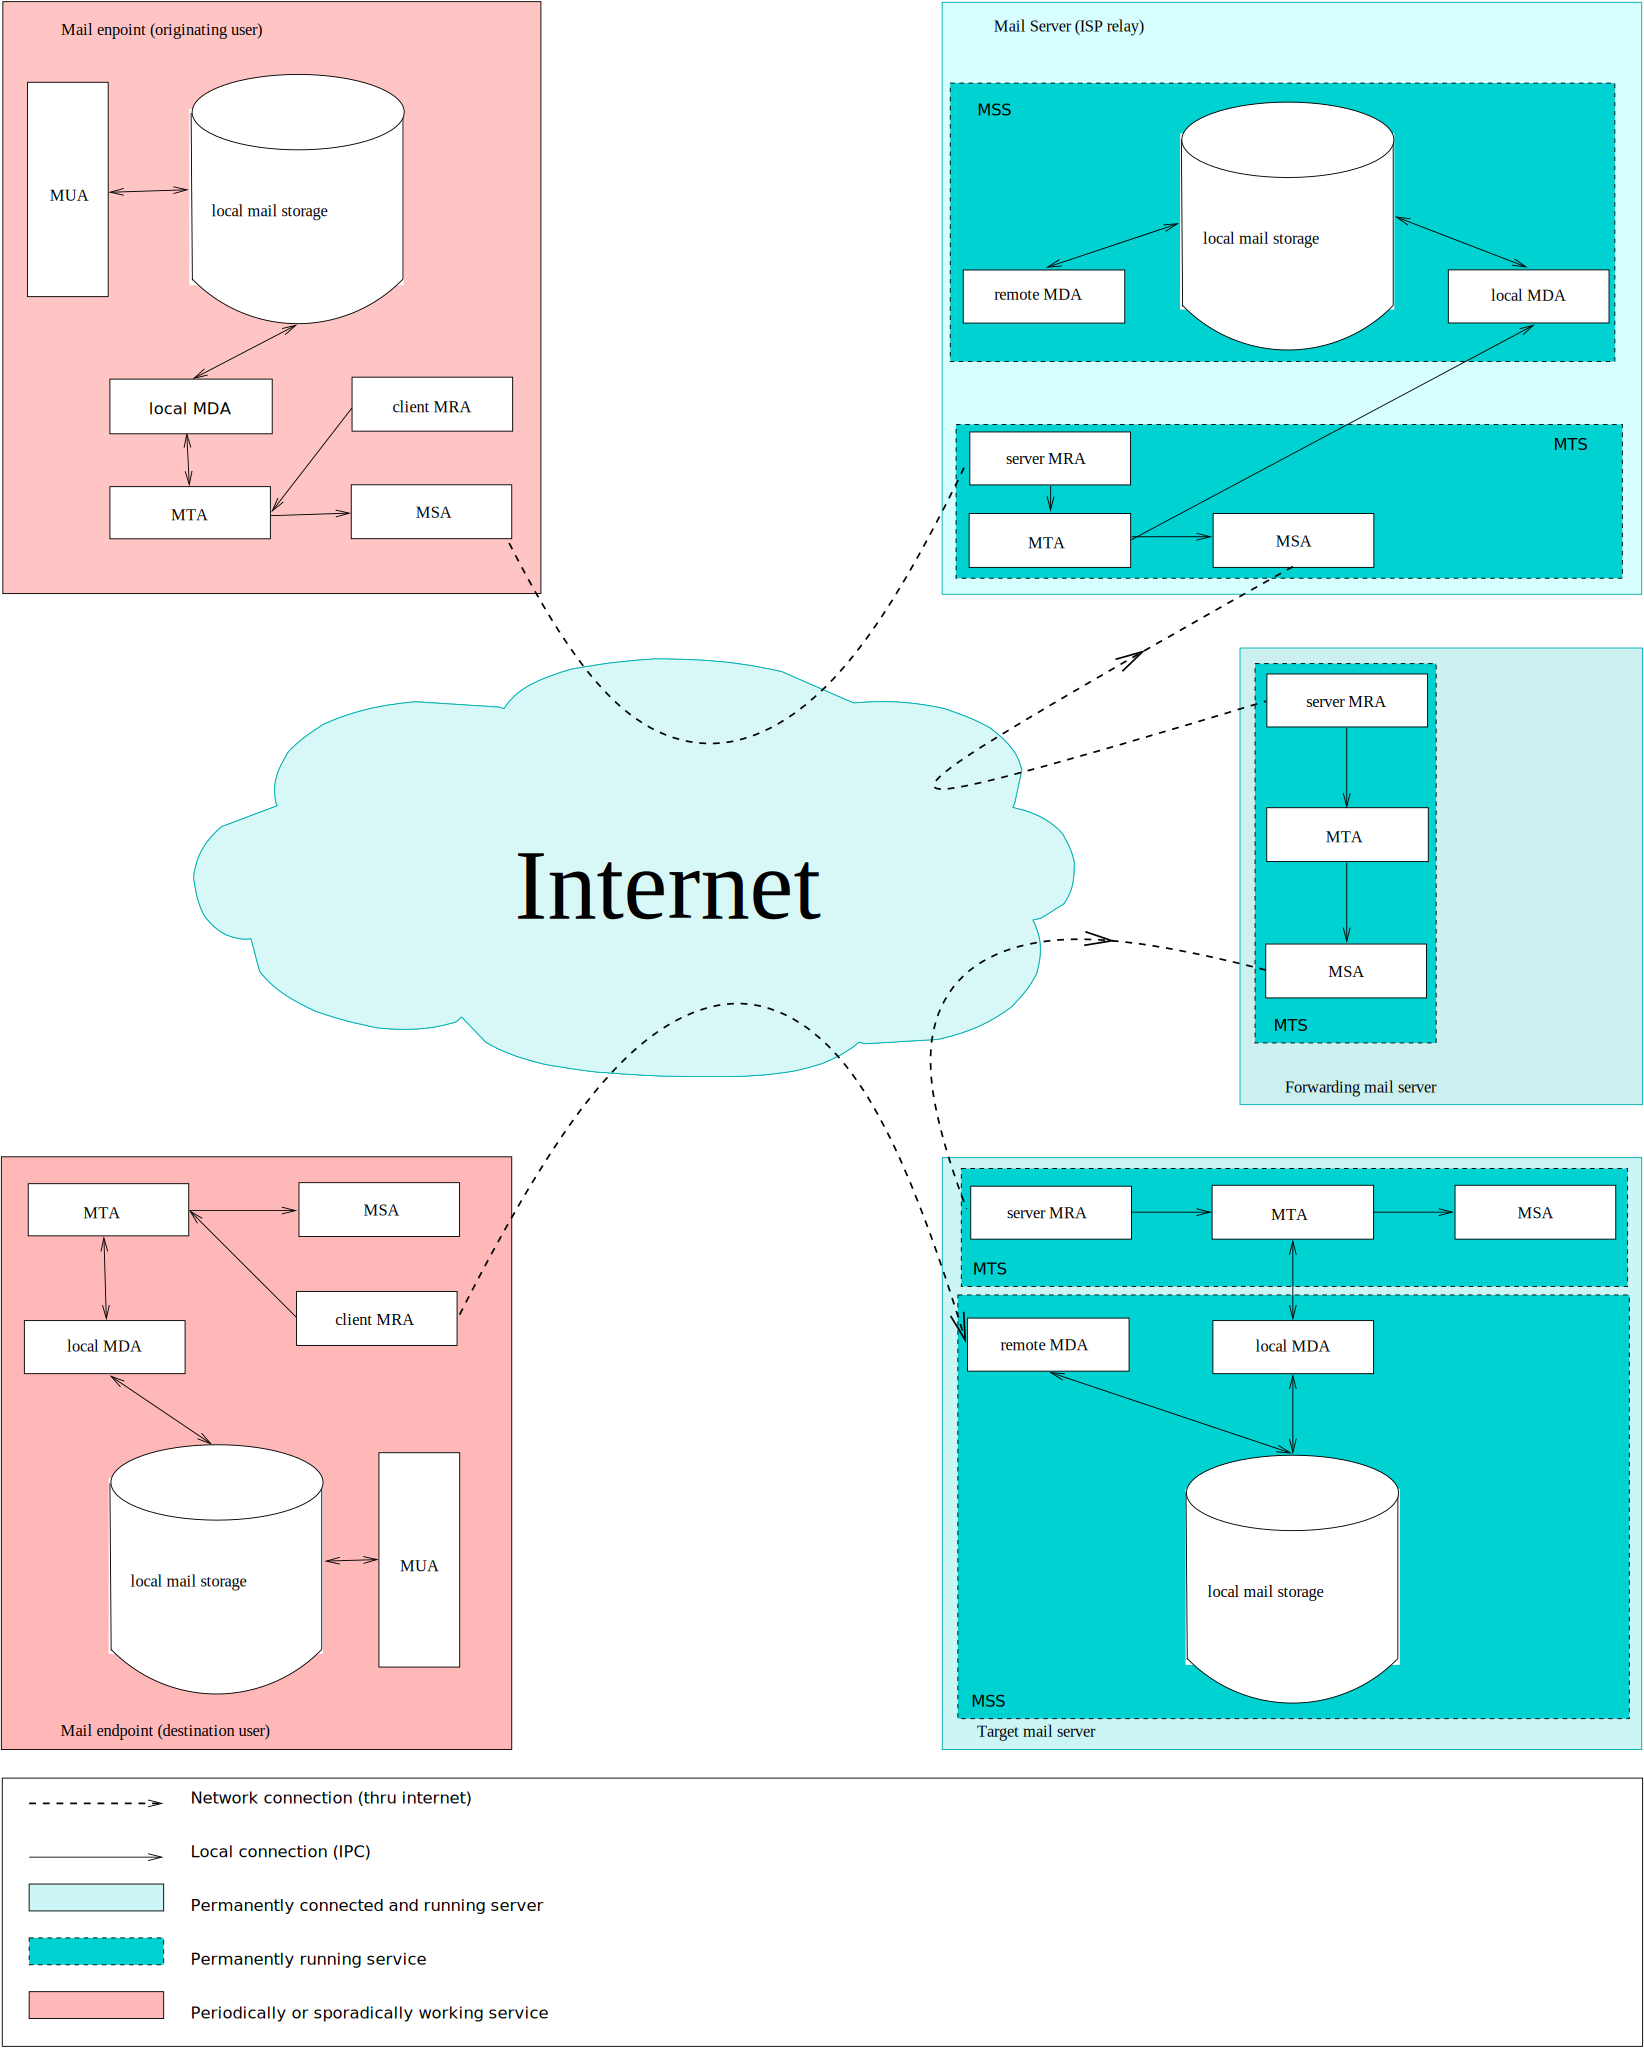
\includegraphics[width=\columnwidth]{inc/MailAgents1.pdf}
	\caption{Mail Agents}\label{fig:MailAgents}
\end{figure}

In the following paragraphs (for definitions), the term ``email'' is used synonymously to the term ``Message''.  ``Email'' has been chosen over ``messages'' because of its frequent use in standard documents.

Emails are typically initiated by a Mail User Agent (\defref{MUA}). An MUA accesses local email storage, which may be the server storage or a local copy. The local copy may be a cache only copy, the only existing storage (when emails are fetched and deleted from the server after retrieval), or a collected representation of multiple server storages (cache or authoritative).

Besides the MUA, the only other component accessing local email storage is the Mail Delivery Agent (\defref{MDA}). An MDA is responsible for storing and fetching emails from the local mail storage. Emails destined for other accounts than the current one are forwarded to the MTA. Emails destined to a User are persistently stored in the local email storage. It is essential to understand that email storage does not necessarily reflect a single mailbox. It may as well represent multiple mailboxes (e.g., a rich client-serving multiple IMAP accounts) or a combined view of multiple accounts (e.g., a rich client collecting mail from multiple \defref{POP} accounts). In the case of a rich client, the local MDA is part of the software provided by the user agent. In the case of an email server, the local MDA is part of the local email store (not necessarily of the mail transport service).

On the server-side, there are usually two components (services) at work. A ``Mail Transport Service'' (\defref{MTS}) responsible for mail transfers and a ``Mail Storage System'' which offers the possibility to store received Mails in a local, persistent store.\par

An MTS generally consists out of three parts. For incoming connects, there is a daemon called Mail Receiving Agent (\defref{Server MRA}) is typically a \defref{SMTP} listening daemon. A Mail Transfer Agent (\defref{MTA}) which is responsible for routing, forwarding, and rewriting emails. Moreover, a Mail Sending Agent (\defref{MSA}) which is responsible for transmitting emails reliably to another Server MRA (usually sent via \defref{SMTP}).\par

An MSS consists of local storage and delivery agents which do offer uniform interfaces to access the local store. They do also deal with replication issues, and grant should take care of the atomicity of transactions committed to the storage. Typically there are two different kinds of \defref{MDA}s. \defref{Local MDA}s offer possibilities to access the store via efficient (non-network based) mechanisms (e.g., IPC or named sockets). This is usually done with a stripped-down protocol (e.g., \defref{LMTP}). For remote agents there a publicly -- network-based -- agent available. Common Protocols for this \defref{Remote MDA}\ include \defref{POP}, \defref{IMAP}, or \defref{MS-OXCMAPIHTTP}.\par

Mail endpoints consist typically of the following components:
\begin{itemize}
	\item A Mail User agent (\defref{MUA})
	\item A Local Mail storage (\defref{MUA})
	\item A Local Mail Delivery Agent (\defref{Local MDA})
	\item A Mail Transfer Agent (\defref{MTA})
	\item A Mail Sending Agent (\defref{MSA})
	\item A Mail Receiving Agent (\defref{MRA})
\end{itemize}

Only two of these components do have external interfaces. These are \defref{MSA} and \defref{MRA}. \defref{MSA} usually uses \defref{SMTP} as transport protocol. When doing so, there are a couple of specialties. 
\begin{itemize}
	\item Port number is 587 (specified in \cite{RFC4409}).\\
	Although port numbers 25 and 465 are valid and do usually have the same capabilities, they are for mail routing between servers only. Mail endpoints should no longer use them.
	\item Connections are authenticated.\\
	Unlike a normal server-to-server (relay or final delivery) SMTP connections on port 25, clients should always be authenticated of some sort. This may be based on data provided by the user (e.g., username/password or certificate) or data identifying the sending system (e.g., IP address)\cite{RFC4409}. Failure in doing authentication may result in this port being misused as a sender for \defref{UBM}.
\end{itemize}

Mail User Agents (MUA) are the terminal endpoint of email delivery. Mail user agents may be implemented as fat clients on a desktop or mobile system or as an interface over a different generic protocol such as HTTP (Web Clients). 

Server located clients are a special breed of fat clients. These clients share the properties of fat clients except for the fact that they do not connect to the server. The client application itself has to be run on the server where the mail storage persists. This makes delivery and communication with the server different. Instead of interfacing with an MSA and a client MDA, they may directly access the local mail storage on the server. On these systems, the local mail storage may be implemented as a database in a user-specific directory structure.

\subsubsection{Fat clients}
The majority of mail clients are fat clients. These clients score over the more centralistic organized web clients in the way that they may offer mail availability even if an Internet connection is not available (through client-specific local mail storage). They furthermore provide the possibility to collect emails from multiple sources and store them in the local storage. Unlike Mail servers, clients are assumed to be not always online. They may be offline most of the time. To guarantee the availability of a particular email address, a responsible mail server for a specific address collects all emails (the \defref{MSS} does this) and provides a consolidated view onto the database when a client connects through a local or remote MDA.

As these clients vary heavily, it is mandatory for the MDA that they are well specified. Lack of doing so would result in massive interoperability problems. Most commonly the Protocols \defref{IMAP}, \defref{POP} and \defref{EWS} are being used these days. For email delivery, the SMTP protocol is used. 

Fat clients are commonly used on mobile devices. According to  \cite{clientDistribution} in Aug 2012 the most typical fat email client was Apple Mail client on iOS devices ($35.6\%$), followed by Outlook ($20.14\%$), and Apple Mail ($11\%$). \citetitle{clientDistribution2}\cite{clientDistribution2} as a more recent source lists in February 2014 iOS devices with $37\%$, followed by Outlook ($13\%$), and  Google Android ($9\%$).

\subsubsection{Server located clients}
Server located clients build an absolute minority. This kind of clients was common in the days of centralized hosts. An example for a Server Located Client is the Unix command ``mail''. This client reads email storage from a file in the users home directory.

\subsubsection{Web clients}
Web clients are these days a common alternative to fat clients. Most big provider companies use their proprietary web client. According to \cite{clientDistribution2} the most common web clients are "`Gmail"', "`Outlook.com"', and "`Yahoo! Mail"'. All these Interfaces do not offer a kind of public plug-in interface. However,  they do offer IMAP-interfaces. This important for a future generalistic approach to the problem.

\section{S/MIME (1996)}
S/MIME is an extension to the MIME standard. The MIME standard allows in simple text-oriented mails an alternate representation of the same content (e.g., as text and as HTML), or it allows to split a message into multiple parts that may be encoded. It is important to note that MIME encoding is only effective in the body part of a mail.

S/MIME, as described in \cite{RFC3851}, extends this standard with the possibility to encrypt mail content or to sign it. Practically this is achieved by either putting the encrypted part or the signature into an attachment. It is essential to know that this method leaks significant pieces of the data.

As the mail travels directly from sender to recipient, both involved parties are revealed. Neither message subject nor message size or frequency is hidden. This method does offer limited protection when assuming an adversary with interest in the message content only. It does not protect from the kind of adversary in our case. 

The trust model is based on a centralistic approach involving generally trusted root certification authorities.

\section{Pretty Good Privacy (1996)}
Exactly as S/MIME PGP\cite{rfc4880} builds upon the base of MIME. Although the trust model in PGP is peer-based. The encryption technology does not significantly differ (as seen from the security model).

Like S/MIME, PGP does not offer anonymity. Sender and endpoints are known to all routing nodes. Depending on the version of PGP, some meta-information or parts of the message content such as subject line, the real name of the sender and receiver, message size is leaked.

A good thing to learn from PGP is that peer-based approaches are offering limited possibilities for trust. The trust in PGP is based on the peer review of users. This peer review may give an idea of how well verified the key of a user is.


% ********************************************************************************************************
% *** Decisions and Research
% ********************************************************************************************************
\part{Substancial Decisions and Research Related to MessageVortex}
\fxwarning{complete section}

MessageVortex is a protocol piggybacking common transport protocols somehow similar as S/MIME\cite{RFC2015} or PGP\cite{PGP} which are common transport protocols such as SMTP. 


\fxwarning{complete intro to the MessageVortex model}

\chapter{Threat Model}
We refer to jurisdiction as a geographical area where a set of legal rules created by a single actor or a group of actors apply, which contains executive capabilities (e.g., police, army, or secret service) to enforce this set of legal rules.

We assume for our protocol that adversaries are state-sponsored actors or players of large organizations. These actors have high funding and expected to have elaborated capabilities themselves or within reach of the sponsor. Actors may join forces with other actors as allies. However, achieving more than 50\% on a world scale is excluded from our model. We always assume one or more actors with disjoint interests covering half of the network or more. 

We assume the following goals for an adversary:
\begin{itemize}
	\item An adversary may want to disrupt non-authorized communication.
	\item An adversary may want to read any information passing through portions of the Internet.
	\item An adversary may want to build and conserve information about individuals or groups of individuals of any aspect of their life. 
\end{itemize}

To achieve these goals, we assume the following properties of our adversary:
\begin{itemize}
	\item An adversary has elaborated technical know-how to attack any infrastructure. This attack may cover any attack favoring his goals, starting with exploiting weaknesses of popular software (e.g., buffer overflows or zero-day exploits) down to simple or elaborated (D)DoS attacks.
	\item An adversary may monitor traffic at any point in public networks within a jurisdiction.
	\item An adversary may modify routing information within a jurisdiction freely.
	\item An adversary may freely modify even cryptographically weak secured data where a single or a limited number of entities grant proof of authenticity or privacy.
	\item An adversary may inject or modify any data on the network of a jurisdiction.
	\item An adversary may create their nodes in a network. He may furthermore monitor their behavior and data flow without limitation.
	\item An adversary may force a limited number of other non-allied nodes to expose their data to him. For this assumption, we explicitly excluded actors with disjoint interests.
	\item An adversary may have similar access to resources as within its jurisdiction in a limited number of other jurisdictions.
\end{itemize}

we may furthermore subdivide the adversaries into the following sub-classes:
\begin{itemize}
	\item A censoring adversary\\
	The primary goal of this adversary is censoring messages and opinions, not within his interests. He does this, regardless of whether the activities of censorship may be observed or not. Therefore, this adversary does not cloak its activities and typically bans censorship circumventing activities as illegal.
	\item An observing adversary\\
	This adversary behaves like a traditional spy. He collects and classifies information while hiding its activities. Unlike within reach of a censoring adversary, in this case, typically, no restrictions apply to the use of anonymization technology.
\end{itemize}


\chapter{Required Properties of our Unobservable Network}
\fxwarning{complete section}
\section{Anonymizing and Unlinking}
\fxwarning{complete section}
\section{Censorship Resistant}
\fxwarning{complete section}
\section{Controllable Trust}
\fxwarning{complete section}
\section{Reliable}
\fxwarning{complete section}
\section{Diagnoseable}
\fxwarning{complete section}
\section{Available}
\fxwarning{complete section}
\section{Identifiable Sender}
\fxwarning{complete section}

\chapter{Identified Problem Hotspots}
\fxwarning{complete section}
\section{Zero Trust Philosophy}
\fxwarning{complete section}
\section{Information leakage and P2P Design}
\fxwarning{complete section}
\section{Accounting}
\fxwarning{complete section}
\section{Anonymisation}
\fxwarning{complete section}
\section{Censorship Resistance}
\fxwarning{complete section}
\section{Initial Bootstraping}
\fxwarning{complete section}
\section{Cypher selection}
\fxwarning{complete section}
\section{Reed-Solomon function}
\fxwarning{complete section}
\section{Usability}
\fxwarning{complete section}
	
\chapter{Protocol}
\fxwarning{complete section}
\section{Key Concepts}
\fxwarning{complete section}
\subsection{Nodes and their Identity Keys}
\fxwarning{complete section}
\subsubsection{Public Vortex Node}
\fxwarning{complete section}
\subsubsection{Hidden Vortex Node}
\fxwarning{complete section}
\subsubsection{Stealth Vortex Node}
\fxwarning{complete section}
\subsection{Protocol Layers}
\fxwarning{complete section}
\subsection{Routing Operations}
\fxwarning{complete section}
\subsection{Vortex Messages}
\fxwarning{complete section}
\subsection{Ephemeral Identities, Workspaces and Accounting}
\fxwarning{complete section}
\subsection{Request and Reply Blocks}
\fxwarning{complete section}
\section{Outline of a Complete MessageVortex Message}
\fxwarning{complete section}
\section{Node Addressing Scheme}
\fxwarning{complete section}


\section{Message Blending}
\fxwarning{complete section}
\subsection{Plain Blending}
\fxwarning{complete section}
\subsection{F5 Blending}
\fxwarning{complete section}

\section{Routing}
\fxwarning{complete section}
\subsection{Algorithms Suitable for Achieving Anonymity}
\fxwarning{complete section}
\subsection{Routing Diagnosis and Reputation Building}
\fxwarning{complete section}
\subsection{Message Path Redundancy}
\fxwarning{complete section}

\section{Protocol Bootstrapping}
\fxwarning{complete section}
\subsection{Key Distribution for Endpoints}
\fxwarning{complete section}
\subsection{Key Aquisition for Routing Nodes}
\fxwarning{complete section}

\chapter{Routing Strategies}
\fxwarning{complete section}
\section{Strictly Onionized Message Routing}
\fxwarning{complete section}
\section{Mixing Routing}
\fxwarning{complete section}
\section{Redundant Message Passing}
\fxwarning{complete section}

\part{Analysis of MessageVortex}
\fxwarning{complete section}
\chapter{Suitability of transport layer protocols}
The following sections list common Internet protocols. We analyze those protocols for the fitness as transport layer of message vortex. 

\section{Methods}
All sections are structured the same way. We first refer to the protocol or standard and describe it in the simplest possible form. We refer to subsequent standards if required to consider extensions where sensible. We then apply the previously referenced criteria and make a concise summary of the suiting of the protocol as a transport layer. The findings of this section is listed in table \ref{tab:protoSuitCrit}. The list here does not reflect the quality or maturity of the protocols. It is a simple analysis of suiting as a transport layer.

All sections are structured the same way. 
\begin{itemize}
	\item Description\\
	We first refer to the protocol or standard and describe it in the simplest possible form. We refer to subsequent standards if required to consider extensions where sensible.
	\item Apply criteria\\\\
	We then apply the previously referenced criteria and make a concise summary of the suiting of the protocol as a transport layer. The findings of this section is listed in table \ref{tab:protoSuitCrit}. The list here does not reflect the quality or maturity of the protocols. It is a simple analysis of suiting as a transport layer.
\end{itemize} 

\subsection{Applied Criteria}
\begin{itemize}
	\item Widely adopted (Ct1)\\
	The more widely adopted and used a protocol is, the harder it is due to the sheer mass for an adversary to monitor , filter, or block the protocol. This is important for censorship resistance of the protocol. 
	\item Reliable (Ct2)\\
	Message transport between peers should be reliable. As messages may arrive anytime from everywhere, we do not have means to synchronize the peer partners on a higher level without investing a considerable effort. Furthermore, the availability of information when what type of information should be available at a specific point in the system would drastically simplify the identification of peers. To avoid synchronization, we do look for inherently reliable protocols.
	\item Symmetrical built (Ct3)\\
	The transport layer should rely on a peer to peer base. All servers implement a generic routing that requires no prior knowledge of all possible targets. This criterion neglects centralized infrastructures. This criterion may be dropped, assuming that the blending layer or a specialized transport overlay is responsible for routing.
\end{itemize}

\subsection{Analyzed Protocols}
We were unable to find a comprehensive list of protocols being used within the Internet and their bandwidth consumption. A weak reference is \cite{zhou2011examining}. This wekaness is founded in the fact that traffic in this report is callified among two critera: Know server or known port. As streaming services consume a considerable part of the Internet bandwidth (acording to the report more than 60\% download). The focus on the report lies on the bandwidth intense figures. However, leavin aside all sources which are strictly one way or dominated by a small number of companies worldwide, the ``top 10'' list of the report shrinks to the two categories ``File sharing'' (Rank 5; 4.2\% download and 30.2\% upload) and ``Messaging'' (Rank 8; 1.6\% download and 8.3\% upload bandwidth). 

In lack of such material we first collected a list of all common Internet messaging protocols (synchronous and asynchronous). We added furthermore some of the most common transfer protocols such as HTTP and FTP and analyzed this list.

\begin{itemize}
	\item Messaging Protocols
	\begin{itemize}
		\item SMTP
		\item CoAP
		\item MQTT
		\item AMQP
		\item XMPP
		\item WAMP
		\item SMS
		\item MMS
	\end{itemize}
	\item Other Protocols
	\begin{itemize}
		\item FTP, SFTP, and FTPS
		\item TFTP
		\item HTTP
	\end{itemize}
\end{itemize}

The following protocols have been discarded as we have considered them as outdated:
\begin{itemize}
	\item MTP\cite{RFC780} (obsoleted by SMTP)
	\item NNTP\cite{RFC3977} (outdated and has only a small usage acording to \cite{kim2010today})
\end{itemize}

We furthermore discarded all RPC-related protocols as they would by definition violate Ct3.

\section{Analysis}
\subsection{HTTP}
The HTTP protocol allows message transfer from and to a server and is specified in RFC2616 \cite{rfc2616}. It is not suitable as a communication protocol for messages due to the lack of notifications. There are some extensions that would allow such communications (such as WebDAV). Still, in general, even those are not suitable as they require a continuous connection to the server to get notifications. Having a ``rollup'' of notifications when connecting is not there by default but could be implemented on top of it. HTTP servers listen on standard ports 80 or 443 for incoming connects. The port 443 is equivalent to the port 80 except for the fact that it has a wrapping encryption layer (usually TLS). The incoming connects (requests) must offer a header part and may contain a body part that would be suitable for transferring messages to the server. The reply to this request is transferred over the same TCP connection containing the same two sections.

HTTP0.9-HTTP/1.1 are clear text protocols which are human-readable (except for the data part which might contain binary data). The HTTP/2\cite{rfc7540} protocol is using the same ports and default behavior. Unlike HTTP/0.9-HTTP/1.1, it is not a clear text but encodes headers and bodies in binary form. 

To be a valid candidate as storage, unauthenticated WebDAV support, as specified in \cite{rfc4918}, must be assumed.

The protocol does satisfy the first two main criteria (Ct1: Widely Adopted and Ct2: Reliable). The main disadvantage in terms of a message transport protocol is that this protocol is not symmetrically. A server is always just ``serving requests'' and not sending information actively to peers. This Request-Reply violates criteria (Ct3: Symmetrically built) and makes the protocol not a primary choice for message transport. 

It is possible to add such behavior to the blending layer using HTTP servers as pure storage. Such a behavior would however be most likely detectable and thus no longer be censorship resistant.

\subsection{FTP}
FTP is defined in RFC959\cite{RFC959}. This Protocol is intended for authenticated file transfer only. There is an account available for general access (``anonymous''). This account does normally not offer upload rights for security reasons. It is possible to use FTP as a message transfer endpoint. The configuration would work as follows: the user ``anonymous'' has upload rights only. It is unable to download or list a directory. A node may upload a message with a random name. In case a collision arises, the node retries with another random name. The blending layer picks messages up using an authenticated user. This workaround has multiple downsides. At first, handling FTP that way is very uncommon and usually requires an own dedicated infrastructure. Such beavior would make the protocol again possibly detectable. Secondly, passwords are always sent in the clear within FTP. Encryption as a wrapping layer (FTPS) is not common, and SFTP (actually a subsystem of SSH) has nothing in common with FTP except for the fact that it may transfer files as well.

Furthermore, FTP may be problematic when used in active mode for firewalls. All these problems make FTP not very suitable as a transport layer protocol. FTPS and SFTP feature similar weaknesses as the FTP version in terms of detectability of non-standard behavior.

Like in HTTP, a disadvantage of FTP in terms of a message transport protocol is that this protocol is not symmetrically. A server is always just ``serving requests'' and not sending information actively to peers. This Request-Reply violates criteria (Ct3: Symmetrically built) and makes the protocol not a primary choice for message transport. The Protocol, however, satisfies the first two criteria  (Ct1: Widely Adopted and Ct2: Reliable).

\subsection{TFTP}
TFTP has, despite its naming similarities to FTP, very little in common with it. TFTP is a UDP based file transfer protocol without any authentication scheme. The possibility of unauthenticated message access makes it not suitable as a transport layer. The protocol is due to the use of UDP in a meshed network with redundant routes. Since the Internet has a lot of these redundant routes, this neglects the use of this protocol.

TFTP is rarely ever used on the Internet, as its UDP based nature is not suitable for a network with redundant routes. Not being common on the Internet violates criterion one (Ct1: Widely Adopted). TFTP is not symmetrically. This means that a server is always just ``serving requests'' and not sending information actively to peers. This Request-Reply violates criteria (Ct3: Symmetrically built) and makes the protocol not a primary choice for message transport. The Protocol furthermore violates Ct2 (Ct2: Reliable) as it is based on UDP without any additional error correction.

\subsection{MQTT}
MQTT is an ISO standard (ISO/IEC PRF 20922:2016) and was formerly called MQ Telemetry Transport. The current standard as the time of writing this document was 3.1.1 \cite{mqtt}. 

The protocol runs by default on the two ports 1883 and 8883 and can be encrypted with TLS. MQTT is a publish/subscribe based message-passing protocol that is mainly targeted to m2m communication. This Protocol requires the receiving party to be subscribed to a central infrastructure in order to be able to receive messages. This makes it very hard to be used in a system without centralistic infrastructure and having no static routes between senders and recipients. 

The protocol does satisfy the second criterion (Ct2: Reliable). It is in the area of end-user (i.e., Internet) not widely adopted, thus violating Criteria 1 (Ct1: Widely Adopted). In terms of decentralization design, the protocol fails as well (Ct3: Symmetrically built).

\subsection{Advanced Message Queuing Protocol (AMQP)}
The Advanced Message Queuing Protocol (AMQP) was initially initiated by numerous exponents based mainly on finance-related industries. The AMQP-Protocol is either used for communication between two message brokers, or between a message broker and a client\cite{amqp}.

It is designed to be interoperable, stable, reliable, and safe. It supports either SASL or TLS secured communication. The use of such a tunnel is controlled by the immediate sender of a message. In its current version 1.0, it does, however, not support a dynamic routing between brokers\cite{amqp}.

Due to the lack of a generic routing capability, this protocol is therefore not suitable for message transport in a generic, global environment.

The protocol satisfies partially the first criterion (Ct1: Widely Adopted) and fully meets the second criterion (Ct2: Reliable). However, the third criterion is violated due to the lack of routing capabilities between message brokers (Ct3: Symmetrically built).

\subsection{Constrained Application Protocol (CoAP)}
The Constrained Application Protocol (CoAP) is a communication Protocol which is primarily destined to m2m communication. It is defined in RFC7252\cite{RFC7252}.  It is defined as a lightweight replacement for HTTP in IoT devices and is based on UDP.

The protocol does partially satisfy the first criteria (Ct1: Widely Adopted). The second criterion (Ct2: Reliable) is only partially fulfilled as it is based on UDP and does only add limited session control on its own.

The main disadvantage in terms of a message transport protocol is that this protocol is not (like HTTP) symmetrically. This means that a server is always just ``serving requests'' and not sending information actively to peers. This Request-Reply violates criteria (Ct3: Symmetrically built) and makes the protocol not a primary choice for message transport. 

\subsection{Web Application Messaging Protocol (WAMP)}
WAMP is a web-sockets based protocol destined to enable M2M communication. Like MQTT, it is publish respectively subscribe oriented. Unlike MQTT, it allows remote procedure calls (RPC).

The WAMP protocol is not widely adopted (Ct1: Widely Adopted), but it is reliable on a per-node base (Ct2: Reliable). Due to its RPC based capability, unlike MQTT, a routing like capability could be implemented. Symmetrical protocol behavior is therefore not available but could be built in relatively easy.

\subsection{XMPP (jabber)}
XMPP (originally named Jabber) is a synchronous message protocol used in the Internet. It is specified in the documents RFC6120\cite{RFC6120}, RFC6121\cite{RFC6120}, RFC3922\cite{RFC3922}, and RFC3923\cite{RFC3923}. The protocol is a very advanced chat protocol featuring numeros levels of security including end-to-end signing and object encryption\cite{RFC3923}. There is also a stream initiation extension for transferring files between endpoints \cite{xep0096}.

It has generic routing capabilities spanning between known and unknown servers. The protocol offers a message retrieval mechanism for offline messages similarily to POP \cite{xep0013}.

The protocol itself seems to be a strong candidate as a transport layer as it is being used actively on the Internet.

\subsection{SMTP}
The SMTP protocol is currently specified in \cite{RFC5321}. It specifies a method to deliver reliably asynchronous mail objects through a specific transport medium (most of the time, the Internet). The document splits a mail object into a mail envelope and its content. The envelope contains the routing information, which is the sender (one) and the recipient (one or more) in 7-Bit ASCII. The envelope may additionally contain optional protocol extension material. 

The content should be in 7-Bit-ASCII (8-Bit ASCII may be requested, but this feature is not widely adopted). It is split into two parts. These parts are the header (which does contain meta-information about the message such as subject, reply address, or a comprehensive list of all recipients), and the body which includes the message itself. All lines of the content must be terminated with a CRLF and must not be longer than 998 characters, excluding CRLF.

The header consists of a collection of header fields. Each of them is built by a header name, a colon, and the data. The exact outline of the header is specified in \cite{RFC5322} and is separated with a blank line from the body. 

\cite{RFC5321} furthermore introduces a simplistic model for SMTP message-based communication. A more comprehensive model is presented in section \nameref{sec:mailTransport} as the proposed model is not sufficient for a detailed end-to-end analysis.

Traditionally the message itself is mime encoded. The MIME messages are mainly specified in \cite{RFC2045} and \cite{RFC2046}. MIME allows to send messages in multiple representations (alternates), and attach additional information (such as possibly inlined images or attached documents). 

SMTP is one of the most common messaging protocols on the Internet (Ct1: Widely Adopted), and it would be devastating for the business of a country if, for censoring reasons, this protocol would be cut off. The protocol is furthermore very reliable as it has built-in support for redundancy and a thorough message design making it relatively easy to diagnose problems (Ct2: Reliable). All SMTP servers usually are capable of routing and receiving messages. Messages going over several servers are common (Ct3: Symmetrically built), so the third criterion may be considered as fulfilled as well.

SMTP is considered a strong candidate as a transport layer.  

\subsection{SMS and MMS}
SMS capability was introduced in the SS7 protocol. This protocol allows the message transfer of messages not bigger than 144 characters. Due to this restriction in size, it is unlikely to be suitable for this type of communication as the keys being required are already sized similarly, leaving no space for Messages or routing information.

The \nth{3} Generation Partnership Project (3GPP) maintains the Multimedia Messaging Service (MMS). This protocol is mainly a mobile protocol based on telephone networks.

Both protocols are not widely adopted within the Internet domain. There are gateways providing bridging functionalities to the SMS/MMS services. However, the protocol itself is insignificant on the Internet itself. 

\subsection{MMS}
 This protocol is just like the SMS protocol accessible through the Internet by using gateways but not directly usable within the Internet.

\section{Results}
We have shown that all common M2M protocols failed mainly at Ct3 as there is no need for message routing. In M2M communication contacting foreign machines is not common. Therefore M2M protocolls are typically using static M2M communication over prepared channels. Such behavior is, however unsuitable for a generic messaging protocol.

Pure storage protocols fail at the same criteria as they typically have a defined set of data sources and data sinks, whereas usually at least the data sources are limited in number. This makes those protocols unsuitable again.

We can clearly state that according to the criteria, only a few protocols are suitable. Table \ref{tab:protoSuitCrit2} on page \pageref{tab:protoSuitCrit} shows that only SMTP and XMPP are suitable protocols. Eventually, similar protocols such as HTTP (with WebDAV) or FTP may be usable as well. 

\begin{table}[h]
	\centering\tiny
	\begin{tabular}{|l|l|l|l|}\hline
		\diaghead{\theadfont protocol Criteria}{Protocol}{Criteria} & \thead{Ct1: Widely adopted}     & \thead{Ct2: Reliable} & \thead{Ct3: Symmetrically built}\\\hline
		HTTP     & $\checkmark$            & $\checkmark$        & $\times$\\              
		FTP      & $\checkmark$            & $\checkmark$        & $\times$\\
		TFTP     & $\times$                & $\times$            & $\times$\\
		MQTT     & \textasciitilde         & $\checkmark$        & $\times$\\              
		AMQP     & \textasciitilde         & $\checkmark$        & $\times$\\
		CoAP     & \textasciitilde         & \textasciitilde     & $\times$\\
		WAMP     & $\times$                & $\checkmark$        & \textasciitilde\\
		XMPP     & $\checkmark$            & $\checkmark$        & $\checkmark$\\
		SMTP     & $\checkmark$            & $\checkmark$        & $\checkmark$\\\hline
	\end{tabular}    
	\caption{comparison of protocols in terms of the suitability as transport layer}
	\label{tab:protoSuitCrit2}
\end{table}

The findings of this short analysis suggested that we should use the two protocols, SMTP and XMPP, for our first standardization. We require at least two to prove that the protocol is agnostic to the transport.

\chapter{Routing Strategy Considerations Related to Security and Anonymity}

\chapter{Identification of Possible Attack Schemes}
\fxwarning{complete section}
\section{Static Attacks}
\fxwarning{complete section}
\subsection{Bugging and Tagging Attacks}
\fxwarning{complete section}
\subsection{Information Leaking related to Information Available to Routing Nodes}
\fxwarning{complete section}
\subsection{Identification of Involved Nodes}
\fxwarning{complete section}
\subsection{Identification of MessageVortex Traffic}
\fxwarning{complete section}
\subsection{Identification of Message Traffic}
\fxwarning{complete section}
\subsection{Identification of Software Updates Traffic}
\fxwarning{complete section}
\section{Dynamic Attacks}
\fxwarning{complete section}
\subsubsection{DoS Attacks Against the Transport System}
\fxwarning{complete section}
\subsection{Attacks Against the Vortex System Itself}
\fxwarning{complete section}
\subsubsection{DoS by Traffic Replay}
\fxwarning{complete section}
\subsubsection{DoS by Traffic Generation}
\fxwarning{complete section}
\subsection{Attacking a Single Ephemeral Identity of a MessageVortex Node}
\fxwarning{complete section}
\subsubsection{Denial of Service by Exhausting Quotas or Limits}
\fxwarning{complete section}
\subsection{Attacking Sending and Receiving Identities of the MessageVortex System}
\fxwarning{complete section}
\subsubsection{Traffic Highlighting or Traffic Analysis}
\subsection{Recovery of Previously Carried Out Operations}
\fxwarning{complete section}

\chapter{Static Security Analysis of the Protocol}
\fxwarning{complete section}
\section{Detection of Transport Layer Messages and Blending}
\fxwarning{complete section}
\subsection{Identification of a Message}
\fxwarning{complete section}
\subsubsection{Plain Embedding}
\fxwarning{complete section}
\subsubsection{F5}
\fxwarning{complete section}
\subsection{Message Structure Related to Censorship Circumvention}
\fxwarning{complete section}
\subsection{Message Structure Related to Information Leaking}
\fxwarning{complete section}
	
\chapter{Dynamic Security Analysis of the Protocol}
\fxwarning{complete section}
\fxwarning{Add timing considerations here}
\section{Attacks Against the Vortex System Itself}
\fxwarning{complete section}
\subsection{DoS Attacks against the System}
\fxwarning{complete section}
\subsection{Attacking a Single Ephemeral Identity of a MessageVortex Node}
\fxwarning{complete section}
\subsection{Attacking Sending and Receiving Identities of the MessageVortex System}
\fxwarning{complete section}
\subsection{Recovery of Previously Carried Out Operations}
\fxwarning{complete section}
\subsection{Attacking Routing Participants}
\fxwarning{complete section}
\subsection{Attacking Anonymity Through Traffic Analysis}
\fxwarning{complete section}
\subsection{Attacking Anonymity Through Timing Analysis}
\fxwarning{complete section}
\subsection{Attacking Anonymity through Throughput Analysis}
\fxwarning{complete section}
\subsection{Attacking Anonymity Through Routing Block Analysis}
\fxwarning{complete section}
\subsection{Attacking Anonymity Through Header Analysis}
\fxwarning{complete section}
\subsection{Attacking Anonymity Through Payload Analysis}
\fxwarning{complete section}
\subsection{Attacking Anonymity Through Bugging}
\fxwarning{complete section}
\subsection{Attacking Anonymity Through Replay Analysis}
\fxwarning{complete section}

\chapter{Analysis of the Degree of Anonymization in Comparison to Other Systems}
\fxwarning{complete section}
\section{Mixnet Based or Onionizing Systems}
\fxwarning{complete section}
\section{DHT-Based Systems}
\fxwarning{complete section}
\section{DC-Based Systems}
\fxwarning{complete section}


\part{Discussion on Results}
\fxwarning{complete section}

\chapter{Summary on Weaknesses Found}
\fxwarning{complete section}

\chapter{Summary on the Research Questions}
\fxwarning{complete section}

\chapter{Further Research}
\fxwarning{complete section}

